\documentclass[11pt,a4paper]{article}
\usepackage[T1]{fontenc}
\usepackage{lmodern}
\usepackage[margin=2.2cm]{geometry}
\usepackage{amsmath,amssymb}
\usepackage{booktabs,tabularx,array}
\usepackage{graphicx}
\usepackage{float}
\usepackage{longtable}
\usepackage{xcolor}
\usepackage{tikz}
\usetikzlibrary{arrows.meta,positioning}
\usepackage[hidelinks]{hyperref}
\def\sectionautorefname{Section}\def\subsectionautorefname{Section}

\definecolor{navy}{HTML}{1F3A5F}
\definecolor{soft}{HTML}{EEF3FA}
\definecolor{todo}{HTML}{FDF1E9}
\definecolor{todoline}{HTML}{EB6834}
\newcommand{\code}[1]{\texttt{\small #1}}
% A box the author fills in: the course does not allow LLM-written analysis or conclusions.
\newcommand{\authorbox}[2]{\par\smallskip\noindent\fcolorbox{todoline}{todo}{\parbox{\dimexpr\linewidth-2\fboxsep-2\fboxrule}{%
  \small\textbf{To be written by the author --- #1}\par\smallskip #2}}\par\smallskip}

% generated by make_figures.py
\newcommand{\cfEeight}{0.353}
\newcommand{\cfEfive}{0.370}
\newcommand{\cfEfour}{0.339}
\newcommand{\cfEnine}{0.345}
\newcommand{\cfEone}{0.377}
\newcommand{\cfEonezero}{0.382}
\newcommand{\cfEseven}{0.353}
\newcommand{\cfEsix}{0.370}
\newcommand{\cfEthree}{0.364}
\newcommand{\cfEtwo}{0.361}
\newcommand{\cfMone}{0.405}
\newcommand{\cfTfive}{0.406}
\newcommand{\cfTone}{0.407}
\newcommand{\cfTsix}{0.430}
\newcommand{\cfTthree}{0.405}
\newcommand{\cfTtwo}{0.393}
\newcommand{\cfVone}{0.370}
\newcommand{\cfVthree}{0.371}
\newcommand{\cfVtwo}{0.381}
\newcommand{\cfWfive}{0.388}
\newcommand{\cfWfour}{0.388}
\newcommand{\cfWone}{0.388}
\newcommand{\cfWsix}{0.397}
\newcommand{\cfWthree}{0.376}
\newcommand{\cfWtwo}{0.385}
\newcommand{\cfXone}{0.387}
\newcommand{\cfXthree}{0.404}
\newcommand{\cfXtwo}{0.381}
\newcommand{\cfYfive}{0.352}
\newcommand{\cfYfour}{0.362}
\newcommand{\cfYone}{0.402}
\newcommand{\cfYthree}{0.397}
\newcommand{\cfYtwo}{0.411}
\newcommand{\cfensone}{0.383}
\newcommand{\cfensseven}{0.419}
\newcommand{\cfenstwo}{0.400}
\newcommand{\cfstackeight}{0.447}
\newcommand{\cfstackfour}{0.422}
\newcommand{\cfstacknine}{0.460}
\newcommand{\cfstackoneone}{0.460}
\newcommand{\cfstackonezero}{0.460}
\newcommand{\cfstackseven}{0.444}
\newcommand{\cfstacksix}{0.423}
\newcommand{\corrfreq}{0.53}
\newcommand{\freqmax}{11,577}
\newcommand{\freqmin}{270}
\newcommand{\fullparams}{88.6M}
\newcommand{\kdinfer}{104}
\newcommand{\kdparams}{63.4M}
\newcommand{\meanensall}{0.408}
\newcommand{\membersteacher}{E2, E3, E5}
\newcommand{\membersteacherfour}{W1, W2, W3, W4, W5, W6, X1, X3}
\newcommand{\membersteacherthree}{W1, W2, W3, W5, W6}
\newcommand{\membersteachertwo}{E1, E3, E6, V2, V3}
\newcommand{\ndevintest}{96}
\newcommand{\ndevintrain}{118}
\newcommand{\ndevraw}{10,181}
\newcommand{\nlabels}{100}
\newcommand{\ntest}{13,019}
\newcommand{\ntrain}{42,315}
\newcommand{\ntraindup}{435}
\newcommand{\ntrainraw}{42,750}
\newcommand{\nval}{10,024}
\newcommand{\nzips}{48}
\newcommand{\rarecount}{30}
\newcommand{\shortereight}{88}
\newcommand{\topshare}{41}

\makeatletter\newcommand{\tabinput}[1]{\@@input #1 }\makeatother % expandable \input inside tabulars

\title{\textbf{CS-781 Capstone, Phase 5: Legal Statute Identification}\\[2pt]
\large A multi-label chunk classifier on the four Phase-1 language models}
\author{Manish Kumar (251330604)\\ CS-781, IIT Kanpur}
\date{October 2026}

\begin{document}
\maketitle

\begin{abstract}
\noindent We assign the relevant statutes (\nlabels{} statute ids, several per document) to Indian legal
documents, starting from the four legal language models pre-trained in Phase~1.  A document is cut into
512-token chunks; eight chunks are encoded by the Phase-1 backbone, read by a BiGRU and pooled by one attention
query per statute.  Ten first-round experiments cover all four architectures and eight adaptation techniques
(full and partial fine-tuning, LoRMA, QLoRA, AdaLoRA, Houlsby adapters, prefix and prompt tuning) plus
knowledge distillation; later rounds train longer and distil from growing ensembles of earlier runs.  All
scores are macro-F1 on a cleaned validation split with per-statute thresholds \emph{cross-fitted} (fitted on one
half, scored on the other).  The best single Phase-1 model is a 6-block A4 student distilled from an 8-model
teacher (\cfYtwo); an MLP stacker over 27 Phase-1 runs reaches \cfstacksix, and a hybrid stacker that adds
lexical TF-IDF models reaches \cfstackoneone.  All numbers are generated from the run outputs by
\code{p5/report/make\_figures.py}.
\end{abstract}

\tableofcontents
\newpage

% =====================================================================
\section{Introduction}
Legal statute identification (LSI) asks which of \nlabels{} statutes apply to a case document; a document can
cite several.  The primary metric is macro-F1 over statutes, so rare statutes weigh as much as frequent ones;
micro-F1 and subset accuracy are secondary.  In this corpus the statute names are masked in the text
(\code{<SECTION>}, \code{<ACT>}), so the model must infer statutes from the facts, not read them off.
The rules require the Phase-1 models as the only pretrained weights, all four architectures, at least six
substantially different experiments with at least five adaptation techniques, LoRMA and knowledge distillation.

% =====================================================================
\section{Data and integrity checks}\label{sec:data}
\begin{table}[H]\centering\small
\caption{Splits used (lengths in Phase-1 BPE tokens).}\label{tab:data}
\begin{tabular}{lrrrrr}\toprule
Split & Documents & Statutes / doc & Median length & 90th pct. & Tokens\\\midrule
\tabinput{tables/data.tex}
\bottomrule\end{tabular}\end{table}

\paragraph{Cleaning} (\code{p5/lsi/data.py}).
\begin{itemize}
  \item \texttt{train.json} has \ntrainraw{} entries; \ntraindup{} are exact duplicates of another entry's text
  (whitespace-normalised hash).  Duplicates are merged and their label sets unioned (80 duplicated texts carry
  different label sets), leaving \ntrain{} training documents.
  \item \texttt{dev.json} (\ndevraw{} documents) contains \ndevintest{} texts that also occur in the test file
  and \ndevintrain{} that occur in training.  They are removed, leaving the \nval{} validation documents used
  for every selection decision.
\end{itemize}
Statute frequencies are long-tailed: the most frequent statute occurs in \freqmax{} training documents, the
rarest in \freqmin, and the ten most frequent account for \topshare\% of all labels (\autoref{fig:labels}).

\begin{figure}[H]\centering
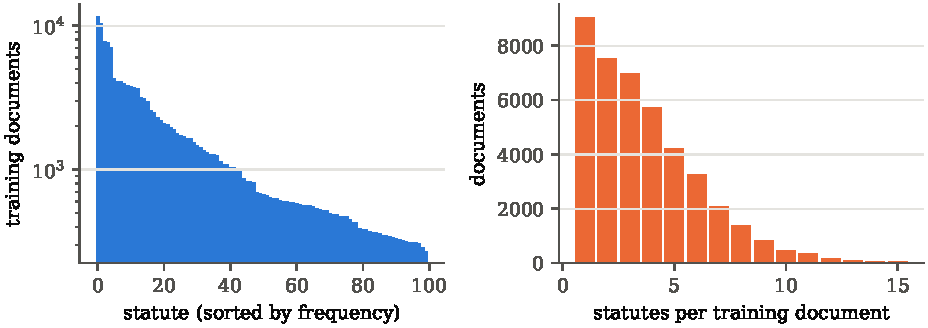
\includegraphics[width=0.95\linewidth]{figs/labels.pdf}
\caption{Left: training documents per statute. Right: statutes per training document.}
\label{fig:labels}\end{figure}

% =====================================================================
\section{Methods}
\subsection{Hierarchical multi-label model}
\begin{figure}[H]\centering
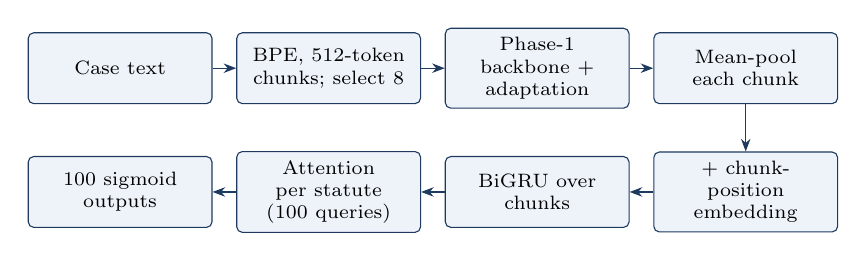
\begin{tikzpicture}[node distance=3mm, box/.style={draw=navy,rounded corners=2pt,fill=soft,align=center,
  font=\scriptsize,minimum height=9mm,text width=21mm}, arr/.style={-{Stealth[length=1.6mm]},navy}]
  \node[box] (a) {Case text};
  \node[box,right=of a] (b) {BPE, 512-token chunks; select 8};
  \node[box,right=of b] (c) {Phase-1 backbone + adaptation};
  \node[box,right=of c] (d) {Mean-pool each chunk};
  \node[box,below=6mm of d] (e) {+ chunk-position embedding};
  \node[box,left=of e] (f) {BiGRU over chunks};
  \node[box,left=of f] (g) {Attention per statute (100 queries)};
  \node[box,left=of g] (h) {100 sigmoid outputs};
  \foreach \x/\y in {a/b,b/c,c/d,d/e,e/f,f/g,g/h} \draw[arr] (\x)--(\y);
\end{tikzpicture}
\caption{The LSI model (\code{p5/lsi/model.py}).}
\label{fig:model}\end{figure}

\begin{itemize}
  \item \textbf{Chunking} (\code{data.strategy}).  Eight chunks of 512 tokens: \emph{spread} evenly over the
  document (default; the whole document when it is at most eight chunks long, \shortereight\% of validation
  documents), or \emph{evidence} (V1): chunks centred on the masked \code{<SECTION>}/\code{<ACT>} placeholders.
  \item \textbf{Document layer}: projection to 384 dimensions, a learned chunk-position embedding, a BiGRU over
  the chunks and \emph{per-statute attention}: each statute has its own query vector over the chunk states
  (a statute is often discussed in one part of the judgment) and its own output vector.
  \item \textbf{Loss}: binary cross-entropy per statute with positive weights $\sqrt{n_\text{neg}/n_\text{pos}}$
  (capped at 30) to give rare statutes more weight.
  \item \textbf{Backbones}: as in Phases 3--4, A1 and A4 keep their causal mask, A3 reads each chunk as a
  bidirectional prefix and A2 uses its decoder states; all start from the cleaned 1B-token Phase-1 checkpoints.
\end{itemize}

\subsection{Adaptation techniques}
\begin{itemize}
  \item \textbf{Full fine-tuning} (E2 A1; later W2/X2 A4, Y4 A3, Y5 A2).
  \item \textbf{Partial fine-tuning} (E4 A2, E5 A4): the top four blocks and the final norm.
  \item \textbf{LoRMA} (E1, W4; A4) \cite{bihany2025lorma}: multiplicative low-rank update
  $W=(I+\tfrac{\alpha}{r}BA)W_0$, $r=16$, $\alpha=32$, on attention and MLP projections.
  \item \textbf{QLoRA} (E6, W5, X1; A1) \cite{dettmers2023qlora}: the frozen backbone stored in 4-bit NF4 (block 64),
  LoRA $r=16$ on top.
  \item \textbf{AdaLoRA} (E7; A3) \cite{zhang2023adalora}: SVD-form update, rank pruned from 12 to 8.
  \item \textbf{Houlsby adapters} (E3, W3; A3) \cite{houlsby2019adapters}: bottleneck 64.
  \item \textbf{Prefix tuning} (E8; A4) \cite{li2021prefix}: 16 learned key/value positions per layer from an MLP.
  \item \textbf{Prompt tuning} (E9; A1) \cite{lester2021prompt}: 20 learned input embeddings.
  \item \textbf{Knowledge distillation} \cite{hinton2015kd} (E10, W6, X3, Y1, Y2, Y3): the student is A4 with 6 of
  its 10 blocks (0, 2, 4, 5, 6, 8; all global-attention layers kept) or A1 with 6 of 8 (Y3), fully fine-tuned with
  $\alpha\,\mathrm{BCE} + (1-\alpha)\,T^2\,\mathrm{BCE}(\sigma(z_s/T), \sigma(z_t/T))$, $T=2$.  The teacher is the
  average logit of an ensemble of earlier runs, computed once on the training set (\code{dump\_logits.py}):
  TEACHER = \membersteacher, TEACHER2 = \membersteachertwo, TEACHER3 = \membersteacherthree, TEACHER4 =
  \membersteacherfour.  Y2 uses $\alpha=0.3$, the others $0.5$.
\end{itemize}

\subsection{Training, selection and thresholds}\label{sec:train}
AdamW, 16 documents per step, 5\% warm-up then cosine decay, weight decay 0.01, gradient clipping 1.0, bf16.
First round: 3 epochs; learning rate $5\times10^{-5}$ for full fine-tuning and KD students, $10^{-4}$ for
partial fine-tuning, $2\times10^{-4}$ for LoRMA, QLoRA, AdaLoRA and adapters, $10^{-3}$ for prefix and
$3\times10^{-3}$ for prompt tuning; the document layer always uses $10^{-3}$.  Later rounds train 5--8 epochs.
Every 800--2{,}000 steps a fixed 2{,}000-document subset of validation is scored and the best state is kept.

\paragraph{Thresholds.} A statute is predicted when its probability exceeds its threshold.  Per-statute
thresholds are chosen on validation (grid search, at least 5 validation positives, else the global
threshold) and every document gets at least one statute.  Because fitting 100 thresholds on the same data
inflates the score, every number in this report is \emph{cross-fitted}: thresholds fitted on one half of
validation score the other half and vice versa (\code{make\_submission.py}).  The test submission uses
thresholds fitted on all of validation.

\subsection{Ensembles and stacking}
\begin{itemize}
  \item \textbf{Mean ensembles} (ENS*): average probability of several runs, members picked greedily on
  validation (\code{ensemble\_select.py}).
  \item \textbf{MLP stacker} (\code{stack.py}): input = the logits of every run for all 100 statutes, one hidden
  layer of 512, dropout 0.3, 30 epochs; trained 5-fold on the validation split, so every validation document is
  scored by a stacker that did not see it; the 5 fold models (and several seeds) are averaged for test.
  \item \textbf{Per-statute GBM stacker} (\code{stack\_gbm.py}): for statute $j$, LightGBM over every run's logit
  for $j$, the mean logit of all statutes and the across-run spread of the logit for $j$; same 5-fold scheme.
  STACK9--11 average the GBM and MLP stackers.
  \item \textbf{Lexical models} (T*, M1): TF-IDF features with one-vs-rest logistic regression or a linear SVM
  (\code{tfidf\_lr.py}), trained on the training split only (T6: on training plus the other validation folds).
  They use no pretrained weights; stacks that include them are reported as \emph{hybrid}.
\end{itemize}

\subsection{Submissions}
\code{make\_submission.py} writes \code{prediction.json}, a list of \code{\{"id", "pred"\}} with the predicted
statute ids for every test document in order, at the root of a zip.

% =====================================================================
\section{Results}
\subsection{All experiments}
\begin{table}[H]\centering
\caption{Validation results (\nval{} documents).  Global = macro-F1 at one tuned global threshold (in-sample);
CF = cross-fitted per-statute thresholds (honest); P, R, micro-F1 and subset accuracy at CF.  Above the line:
first round (3 epochs); below: longer training and distillation rounds.}\label{tab:results}
\resizebox{\linewidth}{!}{\begin{tabular}{lllrrrrrrrrr}\toprule
Run & Arch & Method & Ep. & Trainable & \% & Global & CF & P & R & Micro & Subset\\\midrule
\tabinput{tables/results.tex}
\bottomrule\end{tabular}}\end{table}

\begin{figure}[H]\centering
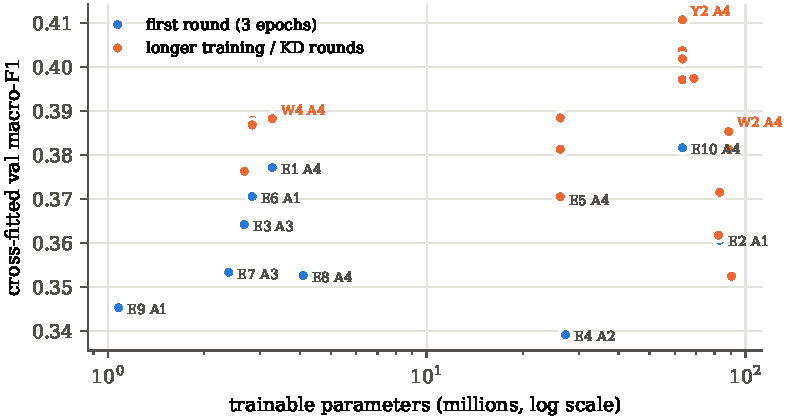
\includegraphics[width=0.85\linewidth]{figs/f1_vs_params.pdf}
\caption{Cross-fitted macro-F1 against the number of trained parameters (document layer included).}
\label{fig:params}\end{figure}

\begin{figure}[H]\centering
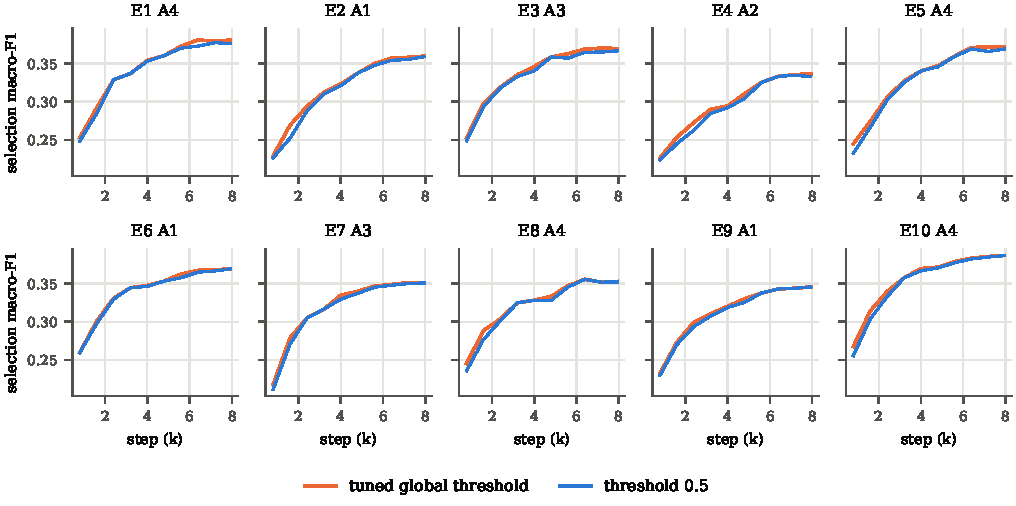
\includegraphics[width=\linewidth]{figs/curves.pdf}
\caption{First-round runs: macro-F1 on the 2{,}000-document selection subset during training.}
\label{fig:curves}\end{figure}

\subsection{Thresholds}
\begin{table}[H]\centering\small
\caption{Threshold strategies on the best single model (Y2).}\label{tab:thr}
\begin{tabular}{lr}\toprule Strategy & Macro-F1\\\midrule
\tabinput{tables/thresholds.tex}
\bottomrule\end{tabular}\end{table}

\subsection{Rare and frequent statutes}
\begin{table}[H]\centering\small
\caption{Y2 per-statute F1 by training-frequency quintile (20 statutes each).  Correlation of per-statute F1
with log frequency: \corrfreq.}\label{tab:perlabel}
\begin{tabular}{llrrrr}\toprule
Quintile & Training docs & Statutes & Mean F1 & Min & Max\\\midrule
\tabinput{tables/perlabel.tex}
\bottomrule\end{tabular}\end{table}

\begin{figure}[H]\centering
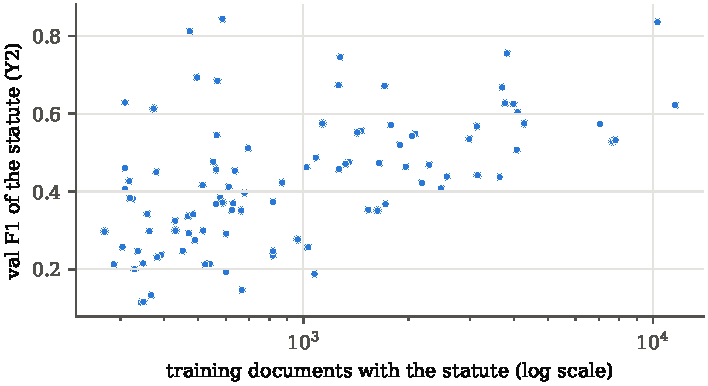
\includegraphics[width=0.75\linewidth]{figs/perlabel.pdf}
\caption{Per-statute validation F1 of Y2 against training frequency.}
\label{fig:perlabel}\end{figure}

\subsection{Missed and confused statutes}
\begin{table}[H]\centering\small
\caption{Y2: frequent statutes (at least the median frequency) with the lowest validation F1.}\label{tab:worst}
\begin{tabular}{rrrrrrr}\toprule
Statute & Train docs & Val docs & F1 & TP & FP & FN\\\midrule
\tabinput{tables/worst.tex}
\bottomrule\end{tabular}\end{table}

\begin{table}[H]\centering\small
\caption{Y2: most frequent (missed gold statute, wrongly predicted statute) pairs in the same validation
document, with how often the two statutes co-occur in training.}\label{tab:conf}
\begin{tabular}{rrrrrr}\toprule
Missed & Predicted & Docs & Train (missed) & Train (predicted) & Co-occur in train\\\midrule
\tabinput{tables/confusions.tex}
\bottomrule\end{tabular}\end{table}

\subsection{Knowledge distillation and efficiency}\label{sec:kdnote}
\begin{table}[H]\centering\small
\caption{Size, compute and memory.  Test inference = seconds to score the \ntest{} test documents.}\label{tab:eff}
\resizebox{\linewidth}{!}{\begin{tabular}{lllrrrrrr}\toprule
Run & Arch & Method & Total & Trainable & Train (min) & Test infer.\ (s) & Peak GB & Ckpt MB\\\midrule
\tabinput{tables/efficiency.tex}
\bottomrule\end{tabular}}\end{table}
The distilled students have \kdparams{} parameters against \fullparams{} for full A4.  The KD chain is
E10 (\cfEonezero) $\rightarrow$ W6 (\cfWsix) $\rightarrow$ X3 (\cfXthree) $\rightarrow$ Y1 (\cfYone) and Y2
(\cfYtwo), each distilled from a larger teacher ensemble; the best non-distilled single run is W4 LoRMA
(\cfWfour).

\subsection{Ensembles, stacking and lexical models}
\begin{table}[H]\centering\small
\caption{Lexical models (no pretrained weights; inputs to the hybrid stacks), cross-fitted.}\label{tab:lex}
\begin{tabular}{llrrr}\toprule Run & Model & Macro-F1 & Micro-F1 & Train (min)\\\midrule
\tabinput{tables/lexical.tex}
\bottomrule\end{tabular}\end{table}

\begin{table}[H]\centering\small
\caption{Ensembles and stackers (cross-fitted / out-of-fold validation scores).  The plain mean of the 27
Phase-1 runs scores \meanensall.}\label{tab:stacks}
\resizebox{\linewidth}{!}{\begin{tabular}{lllrrrr}\toprule
Name & Combination & Inputs & Macro-F1 & P & R & Micro-F1\\\midrule
\tabinput{tables/stacks.tex}
\bottomrule\end{tabular}}\end{table}

\begin{figure}[H]\centering
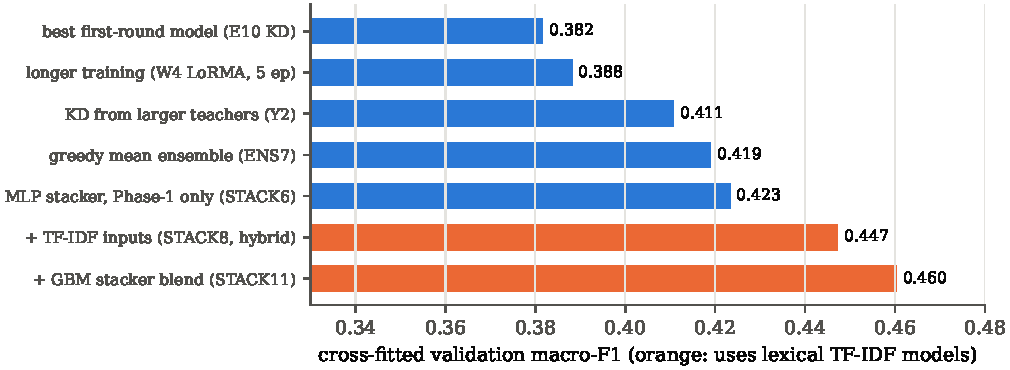
\includegraphics[width=0.9\linewidth]{figs/ladder.pdf}
\caption{Steps from the best first-round model to the final submission.}
\label{fig:ladder}\end{figure}

\subsection{Submission files}
\nzips{} format-checked zips are in \code{p5/submissions/}.  Uploaded first: \code{STACK11\_full} (hybrid,
\cfstackoneone), \code{STACK10\_seedavg} (hybrid), \code{STACK6\_all} (Phase-1 models only, \cfstacksix),
\code{Y2\_kd4\_a4\_alpha03} (best single model, KD) and \code{W4\_a4\_lorma\_ep5} (LoRMA).
\authorbox{leaderboard scores}{Add the Codabench test macro-F1, micro-F1 and subset accuracy of each uploaded
submission and say which six or more count towards the requirement.}
{\scriptsize\begin{longtable}{l}\toprule File\\\midrule\endhead
\tabinput{tables/submissions.tex}
\bottomrule\end{longtable}}

% =====================================================================
\section{Analysis}
\authorbox{analysis of the results}{The course rules do not allow LLM-written result analysis.  Questions the
course asks (§11.5), with the evidence above:
\begin{itemize}
  \item Which adaptation techniques are effective for LSI, and can parameter-efficient methods retain full
  fine-tuning performance (\autoref{tab:results}, \autoref{fig:params})?
  \item How do long-document representation strategies affect statute identification (spread vs.\ evidence
  chunks: E5 vs.\ V1)?
  \item How do rare statutes affect performance (\autoref{tab:perlabel}, \autoref{fig:perlabel})?
  \item Which loss and class-balancing strategies are useful (positive weights, \autoref{sec:train})?
  \item How do threshold strategies affect precision, recall and macro-F1 (\autoref{tab:thr})?
  \item Do multi-label relationships help (per-statute attention; the stackers' all-statute inputs,
  \autoref{tab:stacks})?
  \item Which statutes are commonly missed or confused (\autoref{tab:worst}, \autoref{tab:conf})?
  \item Is information from particular sections of the document useful?
  \item Does distillation keep performance while reducing size and compute (\autoref{tab:eff})?
  \item How do model size, memory and inference cost change across experiments?
  \item Are the Phase-1 representations useful for LSI (compare with the lexical models, \autoref{tab:lex})?
\end{itemize}}

\section{Limitations and next steps}
Facts that limit the conclusions (the interpretation is the author's):
\begin{itemize}
  \item One seed per run; runs differ by a few thousandths of macro-F1, which is within seed noise.
  \item Stackers are trained on the validation split (5-fold); their scores are out-of-fold, but stacker
  settings were chosen on the same split.
  \item The best submissions (STACK7--11) include lexical TF-IDF models that use no Phase-1 weights; STACK6 is
  the best Phase-1-only combination.
  \item Eight 512-token chunks cover the whole document for \shortereight\% of validation documents.
  \item Statute names are masked, which removes the lexical shortcut but also the most direct evidence.
\end{itemize}
\authorbox{what you would do next}{With more time or compute: \ldots}

\section{Conclusions}
\authorbox{conclusions}{Summarise what you conclude from the experiments, in your own words.}

\section{Reproducibility}
\noindent{\small\begin{tabularx}{\linewidth}{l>{\raggedright\arraybackslash}X}
Token cache & built on first use by \code{lsi/data.py} (\code{build\_cache})\\
First-round experiments & \code{bash run\_queue.sh}\\
One experiment & \code{python train.py --config configs/w4\_a4\_lorma\_ep5.yaml}\\
Teacher logits + KD & \code{python dump\_logits.py --run runs/W1\_a4\_partial\_ep8 ... --out TEACHER4\_ens};
\code{python train.py --config configs/y2\_kd4\_a4\_alpha03.yaml}\\
Single-run zip & \code{python make\_submission.py --run runs/Y2\_kd4\_a4\_alpha03}\\
Lexical models & \code{python tfidf\_lr.py --name T1\_tfidf\_word ...}\\
Stackers & \code{python stack.py --all --name STACK6\_all}; \code{python stack\_gbm.py --name ... --blend ...}\\
Figures and tables & \code{python p5/report/make\_figures.py}\\
\end{tabularx}}
\authorbox{repository link}{GitHub: \url{https://github.com/...}}

\section*{LLM declaration}
\authorbox{LLM declaration (mandatory)}{Fill in the course questionnaire.  Describe honestly which parts used
an LLM assistant (for example the data pipeline, model and training code, figures and this report's
methods/results text) and which parts are your own (design decisions, hyperparameters, analysis, conclusions).}

\begin{thebibliography}{99}\small
\bibitem{bihany2025lorma} H.~Bihany, S.~Patel, A.~Modi. LoRMA: Low-rank multiplicative adaptation for LLMs. Findings of ACL 2025.
\bibitem{dettmers2023qlora} T.~Dettmers et al. QLoRA: Efficient finetuning of quantized LLMs. NeurIPS 2023.
\bibitem{hinton2015kd} G.~Hinton, O.~Vinyals, J.~Dean. Distilling the knowledge in a neural network. arXiv:1503.02531, 2015.
\bibitem{houlsby2019adapters} N.~Houlsby et al. Parameter-efficient transfer learning for NLP. ICML 2019.
\bibitem{lester2021prompt} B.~Lester, R.~Al-Rfou, N.~Constant. The power of scale for parameter-efficient prompt tuning. EMNLP 2021.
\bibitem{li2021prefix} X.~L.~Li, P.~Liang. Prefix-tuning: Optimizing continuous prompts for generation. ACL 2021.
\bibitem{zhang2023adalora} Q.~Zhang et al. AdaLoRA: Adaptive budget allocation for parameter-efficient fine-tuning. ICLR 2023.
\end{thebibliography}
\end{document}
